\chapter{Implementación}

En este capítulo se describe el proceso de implementación junto con todos los elementos en los que éste se apoya, una descripción de todas las elecciones técnicas tomadas junto con su justificación.

En primer lugar se muestra el listado de las historias de usuario generadas junto con sus correspondientes tareas, que dan forma a las unidades de trabajo refinadas. Tras esto, se encuentran todos los dilemas tecnológicos considerados, junto con la solución seleccionada y  una lista de alternativas brevemente definidas con el fin de proveer una justificación fundada y válida de la elección tomada.

\section{Historias de usuario}

Las historias de usuario se usan para definir los beneficios que ciertos tipos de usuarios desean obtener en determinadas situaciones. Cada una de estas historias de usuario representa un avance en la funcionalidad del sistema, y su desarrollo se compone de una a varias tareas.

Partiendo de los requisitos previamente listados, refinándolos en historias de usuario, se puede dar paso a la elaboración de tareas que guíen la implementación del proyecto. Cabe aclarar que, como este desarrollo sigue una mentalidad ágil, las historias y tareas se han ido generando a corto plazo, por lo que la siguiente lista de historias de usuario y sus tareas se ha ido construyendo a lo largo del proceso de desarrollo.

Algunas historias, como ya se verá a continuación, son técnicas. Esto se debe a que lo que se pretende lograr con ellas no encaja del todo en la definición de historia de usuario, pero sin embargo se dividen en tareas igualmente y su implementación es lo suficientemente relevante como para mencionarlas como parte del desarrollo de un PMV.

Así mismo cabe mencionar que el primer \textit{milestone} del proyecto se excluye de esta sección, pues está compuesto únicamente de documentación no directamente relacionada con las tareas de implementación.

\subsection{PMV-1. Gestión básica de libros y bibliotecas.}

\begin{itemize}
    \item \href{https://github.com/Anglepi/My-Many-Reads/issues/29}{\textbf{HU-1}} Solicitar información de libros \\
    Como Sergio, lector en MMR, \\
    quiero solicitar información sobre libros de una base de datos, \\
    con el fin de saber si me pueden interesar según sus características.
    \begin{itemize}
        \item \href{https://github.com/Anglepi/My-Many-Reads/issues/31}{\textbf{T-1.1}} Definir estructura básica de datos para los libros.
        \item \href{https://github.com/Anglepi/My-Many-Reads/issues/32}{\textbf{T-1.2}} Crear primera aproximación de BD de libros.
        \item \href{https://github.com/Anglepi/My-Many-Reads/issues/33}{\textbf{T-1.3}} Métodos para tratar las propiedades de los libros.
    \end{itemize}
    \item \href{https://github.com/Anglepi/My-Many-Reads/issues/30}{\textbf{HU-2}} Bibliotecas para gestionar lecturas
    Como Sergio, lector en MMR, \\
    quiero diferentes colecciones de libros de mi elección, \\
    con el fin de gestionar mis lecturas bajo mis propios criterios.
    \begin{itemize}
        \item \href{https://github.com/Anglepi/My-Many-Reads/issues/34}{\textbf{T-2.1}} Definir estructura básica de datos para las bibliotecas.
        \item \href{https://github.com/Anglepi/My-Many-Reads/issues/35}{\textbf{T-2.2}} Funcionalidad básica de gestión de bibliotecas.
    \end{itemize}
\end{itemize}

\subsection{PMV-2. Implementación de la API y sistema de recomendaciones}
\label{pmv2}

\begin{itemize}
    \item \href{https://github.com/Anglepi/My-Many-Reads/issues/45}{\textbf{HT-3}} Creación de la API. \\
    Es necesario tener una API para realizar todas las tareas de consulta y tratamiento de datos pertinentes sobre las entidades del sistema. \\
    Se utilizara tanto para alimentar el sistema web que se desarrolle en el futuro como para \\
    permitir a los consumidores de información realizar sus consultas.
    \begin{itemize}
        \item \href{https://github.com/Anglepi/My-Many-Reads/issues/46}{\textbf{T-3.1}} Escoger un framework para la API e implementar un ejemplo de uso.
        \item \href{https://github.com/Anglepi/My-Many-Reads/issues/47}{\textbf{T-3.2}} \textit{Endpoints} para los libros.
        \item \href{https://github.com/Anglepi/My-Many-Reads/issues/48}{\textbf{T-3.2}} \textit{Endpoints} para las bibliotecas.
    \end{itemize}
    \item \href{https://github.com/Anglepi/My-Many-Reads/issues/49}{\textbf{HU-4}} Sistema de recomendaciones manuales. \\
    Como Sergio, lector en MMR, \\
    quiero relacionar dos libros mediante una recomendación personal, \\
    con el fin de ayudar a otros usuarios a elegir sus lecturas.
    \begin{itemize}
        \item \href{https://github.com/Anglepi/My-Many-Reads/issues/57}{\textbf{T-4.1}} Determinar e implementar la mejor estructura de datos para recomendaciones creadas por usuarios.
        \item \href{https://github.com/Anglepi/My-Many-Reads/issues/58}{\textbf{T-4.2}} Implementar funcionalidades requeridas para las recomendaciones creadas por usuarios.
        \item \href{https://github.com/Anglepi/My-Many-Reads/issues/59}{\textbf{T-4.3}} Habilitar funcionalidades de las recomendaciones creadas por usuarios en la API.
    \end{itemize}
    \item \href{https://github.com/Anglepi/My-Many-Reads/issues/50}{\textbf{HU-5}} Sistema de recomendaciones automático. \\
    Como Sergio, lector en MMR, \\
    quiero consultar recomendaciones en base a una de mis bibliotecas, \\
    con el fin de ayudarme a decidir mis lecturas.
    \begin{itemize}
        \item \href{https://github.com/Anglepi/My-Many-Reads/issues/66}{\textbf{T-5.1}} Encontrar una estructura de datos que represente la recopilación de características de los libros de una biblioteca.
        \item \href{https://github.com/Anglepi/My-Many-Reads/issues/67}{\textbf{T-5.2}} Medir el nivel de correlación entre un libro y una biblioteca, de acuerdo a sus características recopiladas, para calcular su nivel de similitud.
        \item \href{https://github.com/Anglepi/My-Many-Reads/issues/68}{\textbf{T-5.3}} Crear una lista de recomendaciones a partir de una librería y un conjunto de libros.
    \end{itemize}
    \item \href{https://github.com/Anglepi/My-Many-Reads/issues/76}{\textbf{HT-6}} Capa de gestión de datos. \\
    Es necesario incluir un nuevo componente que haga las veces de conector hacia una base de datos remota. \\
    Este componente debería encargarse de gestionar todas las consultas a la base de datos, ya que no es responsabilidad de la API.
    \begin{itemize}
        \item \href{https://github.com/Anglepi/My-Many-Reads/issues/77}{\textbf{T-6.1}} Crear la estructura básica del gestor de datos.
        \item \href{https://github.com/Anglepi/My-Many-Reads/issues/78}{\textbf{T-6.2}} Añadir al gestor la funcionalidad relevante para las consultas sobre libros.
        \item \href{https://github.com/Anglepi/My-Many-Reads/issues/79}{\textbf{T-6.3}} Añadir al gestor la funcionalidad relevante para las consultas sobre bibliotecas.
        \item \href{https://github.com/Anglepi/My-Many-Reads/issues/80}{\textbf{T-6.4}} Añadir al gestor la funcionalidad relevante para las consultas sobre recomendaciones.
    \end{itemize}
    \item \href{https://github.com/Anglepi/My-Many-Reads/issues/76}{\textbf{HT-7}} Base de datos persistente. \\
    Hasta ahora la base de datos se inicializaba de nuevo con cada ejecución. \\
    Para lograr persistencia, se propone implementar el uso de una base de datos externa que almacene y recupere la información en memoria secundaria.
    \begin{itemize}
        \item \href{https://github.com/Anglepi/My-Many-Reads/issues/77}{\textbf{T-7.1}} Encontrar posibles opciones y escoger la mejor de ellas.
        \item \href{https://github.com/Anglepi/My-Many-Reads/issues/78}{\textbf{T-7.2}} Crear un script que defina las estructuras de las tablas en la base de datos, así como algunos datos de prueba.
        \item \href{https://github.com/Anglepi/My-Many-Reads/issues/79}{\textbf{T-7.3}} Modificar el gestor de datos para que realice la conexión a esta nueva base de datos.
    \end{itemize}
    \item \href{https://github.com/Anglepi/My-Many-Reads/issues/98}{\textbf{HU-8}} Evitar posibles inconsistencias. \\
    Como Sergio, lector en MMR, \\
    quiero que la información y funcionalidades sean consistentes tras cada operación, \\
    con el fin de evitar situaciones inesperadas causadas por mis acciones.
    \begin{itemize}
        \item \href{https://github.com/Anglepi/My-Many-Reads/issues/93}{\textbf{T-8.1}} Evitar entradas duplicadas en las bibliotecas.
        \item \href{https://github.com/Anglepi/My-Many-Reads/issues/94}{\textbf{T-8.2}} Añadir información de cara al usuario sobre el tratamiento de datos en \textit{My Many Reads}.
        \item \href{https://github.com/Anglepi/My-Many-Reads/issues/96}{\textbf{T-8.3}} Usar un identificador único para identificar los libros, evitando el uso del ISBN.
    \end{itemize}
\end{itemize}

\section{Entorno de desarrollo}

A continuación se describen todos los elementos que conforman el entorno de desarrollo, justificando las elecciones tomadas enfrentándolas a las alternativas encontradas e indicando el por qué de la decisión en base a la naturaleza de este proyecto.

\subsection{Gestor de tareas}

Un gestor de tareas permitirá automatizar ciertas tareas relacionadas con el desarrollo de manera más sencilla, como generación de documentación, ejecución de tests, etc. a través de un sencillo comando definido por el desarrollador.


\textbf{Alternativa principal:} \href{https://www.pyinvoke.org/}{\textit{invoke}}.

Muchas de las alternativas se investigaron una vez se tomó la elección del lenguaje de programación a usar, ya que en muchas ocasiones el gestor de tareas depende del lenguaje o funciona particularmente bien junto a éste. 

En cuanto a los gestores de tareas genéricos, la mayoría los acababa descartando, principalmente debido a la sintaxis que empleaban o a que requerían la instalación de complementos adicionales que, probablemente, no usaría para otra cosa, por lo que me pareció inconveniente.

\textit{Invoke} es una muy buena herramienta para gestión de tareas en Python. Mediante un fichero \textit{tasks.py} se definen las tareas a realizar, y dado que la sintaxis de python es muy conocida y para nada compleja, no es difícil de construir. Además se pueden ejecutar órdenes en la línea de comandos muy fácilmente, por lo que también es muy versátil.

Muy probablemente habría sido la opción principal si se supiera desde el principio que se usaría Python para desarrollar el proyecto, dado que no tiene absolutamente nada que envidiarle a \textit{make}. Sin embargo éste se usaba desde el principio del proyecto, y dado que el cambio no aportaba ningún beneficio, se optó por descartar la opción.

\textbf{Elección final:} \href{https://www.gnu.org/software/make/}{\textit{make}}.

\textit{Make} es uno de los gestores de tareas más populares actualmente, muy probablemente debido a la sencillez de su uso e instalación y su versatilidad. El factor determinante para tomar esta decisión fue, principalmente, esta versatilidad, pues sabía que no solo lo usaría para gestionar actividades del desarrollo, sino para todo lo relacionado con la elaboración de este proyecto, incluida la documentación.

Esta elección fue de las primeras que hubo de tomarse, mucho antes de comenzar el desarrollo, pues como es lo habitual, el proyecto comenzó por una documentación e investigación que sirviera para justificar la viabilidad del mismo, sin ser muy relevantes los detalles técnicos del mismo.

Solo es necesario un fichero \href{https://github.com/Anglepi/My-Many-Reads/blob/main/Makefile}{\textit{Makefile}} en el que incluir las tareas a automatizar bajo sus nombres.

\subsection{Editor de código}
\label{Editor de código}

Una vez seleccionado el lenguaje, la opción más común suele ser escoger uno de los \textit{IDEs} disponibles, pues hacen más cómodo el desarrollo. Sin embargo, esta decisión es más subjetiva puesto que no afecta directamente al software producido.

En este caso, se ha optado más por un editor de código que un IDE, por gustos personales más el hecho de centralizar todo el trabajo en una misma aplicación, además de por transparencia con las acciones realizadas y, cómo no, simple costumbre.

\textbf{Alternativa principal:} \href{https://www.sublimetext.com/}{\textit{Sublime Text}}.

Es un editor muy popular, que además recibe actualizaciones de manera frecuente con notables mejoras.

Una de sus ventajas es que no consume tantos recursos, pero dado que tengo la suerte de trabajar en una máquina de buenas prestaciones, este aspecto realmente no me supone un beneficio.

Por otra parte, lo que me hizo descartar esta opción fue el proceso de búsqueda e instalación de complementos, que es bastante manual y tediosa, así como la ausencia de una terminal en el entorno de forma nativa.

Cabe destacar que existen otras alternativas, IDEs para Python, que también pueden considerarse, como \href{https://docs.python.org/3/library/idle.html}{\textit{IDLE}}, que viene integrado, o \href{https://www.jetbrains.com/es-es/pycharm/}{\textit{PyCharm}} de \textit{JetBrains}, un equipo muy conocido por desarrollar muy buenos IDEs.

Un \textit{IDE} sería ideal si solo se fuera a trabajar en código, pero dado que este proyecto también requiere de documentación y podría incluir una variedad de tecnologías a emplear, un simple editor de código con complementos es mucho más adecuado.

\textbf{Elección final:} \href{https://code.visualstudio.com/}{\textit{Visual Studio Code}}.

Es el editor más potente y, desgraciadamente, eso se nota cuando se utiliza en máquinas de bajas prestaciones. Sin embargo, ofrece muchísimas opciones de configuración base, detecta una gran cantidad de lenguajes a los que provee de un formato visual de apoyo y es propiedad de \textit{Microsoft}, por lo que se espera un buen mantenimiento y actualizaciones frecuentes.

Destaca principalmente por ofrecer de forma nativa una terminal, que aunque por defecto usa la nativa del sistema en el que se encuentre instalado, es muy sencillo instalar y usar cualquier otra. Además existe una gama muy amplia de complementos gratuitos y desarrollados por la comunidad, muy fáciles de instalar y gestionar. 

El propio editor te ofrece sugerencias cuando detecta el entorno en el que estás trabajando, y ni si quiera es necesario recurrir al navegador web para consultar información de éstos o instalarlos, pues su gestor de complementos ya satisface todas estas necesidades. Algunos de estos complementos útiles para el proyecto son:
\begin{itemize}
    \item \href{https://marketplace.visualstudio.com/items?itemName=ms-python.python}{Python}, que ofrece características propias del lenguaje como \textit{linting}, \textit{debugging} y formateo de código.
    \item \href{https://marketplace.visualstudio.com/items?itemName=eamodio.gitlens}{GitLens}, que aumenta las funcionalidades relacionadas con Git en el editor.
\end{itemize}

\subsection{Lenguaje de programación}

Para esta decisión, el criterio principal es las capacidades del lenguaje en cuanto a la facilidad que ofrece para implementar las tareas necesarias (paquetes, módulos, complementos, etc.) junto con la eficiencia del mismo y la mantenibilidad a largo plazo.

Por otra parte también se tiene en cuenta un componente subjetivo, pues se valora la comodidad del desarrollador con dicho lenguaje y las filosofías que éste trae consigo.

\textbf{Alternativa:} \href{https://go.dev/}{\textit{Go}}.

Me he decantado por poner esta alternativa ya que es la que tenía en mente al comienzo del proyecto. Sintácticamente es un lenguaje que me encanta, además del control de punteros explícito y otras características, y ya lo había probado anteriormente para desarrollar una API REST y me gustó bastante. Además, tiene al equipo de Google detrás, por lo que inspira bastante confianza.

Es cierto que la \href{https://benchmarksgame-team.pages.debian.net/benchmarksgame/index.html}{velocidad del lenguaje} es importante, pero también lo son las utilidades que ofrece y el nivel de mantenimiento y actualizaciones que prolonga su ciclo de vida.

Demuestra ser bastante más rápido que, por ejemplo, Python en \href{https://benchmarksgame-team.pages.debian.net/benchmarksgame/fastest/go-python3.html}{bastantes situaciones}, pero por desgracia no encontré librerías prometedoras con utilidades para el tratamiento de datos que me permitieran, entre otras cosas, establecer correlaciones.

\textbf{Elección final:} \href{https://www.python.org/}{\textit{Python 3}}.

En un principio mi intención era tomar esta elección dándole bastante importancia a lo cómodo que me sentiría con un lenguaje en cuanto a gustos personales, ya que prefiero lenguajes tipados y más explícitos. Sin embargo, cuanto más avanzaba en las fases de diseño, más peso daba al sistema de recomendación. 

Es evidente que necesitaría algún tipo de API para servir los datos, pero por otra parte también necesitaría buenas herramientas de tratamiento y análisis de datos para poder construir un buen algoritmo de recomendaciones automático. Esto me llevó a pensar que probablemente el lenguaje que buscaba fuera bastante popular, pues habría tener buenas bibliotecas de desarrollo de APIs y de tratamiento de datos, las cuales suelen estar relacionadas con una buena comunidad de desarrolladores.

La decisión, como se indica arriba, fue Python. Este lenguaje he de admitir que no se adapta mucho a mis gustos personales en cuanto a sintaxis y entorno de paquetes, pero lo que ofrece me será de gran utilidad para este desarrollo.

Para evitar algunos posibles errores y apoyar la producción de código más legible, he instalado en mi entorno de desarrollo el \textit{linter} \href{http://mypy-lang.org/}{\textit{mypy}}, con algunas \href{https://github.com/Anglepi/My-Many-Reads/blob/main/.mypy.ini}{reglas configuradas} para hacer la revisión más estricta. Este \textit{linter} fuerza que las funciones y argumentos tengan los tipos correctos, con lo que se consigue algo así como crear un \textit{typescript} de Python.

Éste no es el único \textit{linter} viable. Una de las ventajas de Visual Studio Code es que te ofrece herramientas para seleccionar diferentes \textit{linters} y gestiona su instalación por ti, ofreciéndote las recomendaciones más populares. Cada una de estas suele destacar por centrase en algún aspecto, como por ejemplo \href{https://pypi.org/project/pylint/}{\textit{pylint}}, que se centra en la calidad del código y ofrece sugerencias para refactorizar con respecto a los estándares, y sin ningún problema se puede usar junto a \textit{mypy}, por lo que no es mala idea instalarlo también, con algo de \href{https://github.com/Anglepi/My-Many-Reads/blob/main/.pylintrc.ini}{configuración}.

\subsection{Gestor de dependencias}

Esta es una de las espinitas que tengo clavadas con respecto a Python. La gestión de dependencias es bastante tediosa, y si no se hace bien, puedes crear bastante caos en tu entorno de desarrollo.

En cuanto a gestores de dependencias, aquellos que hayan trabajado con Python sabrán que existen una multitud de opciones diferentes, y cada cuál se escogía por mero gusto personal, por lo que por ahí circulan multitud de proyectos cada uno siendo gestionado e instalado de diferente manera.

Finalmente se ha ido consensuando una buena práctica para estas gestiones, por lo que ésta ha de ser tenida en cuenta.

\textbf{Alternativa:} \href{https://pipenv-es.readthedocs.io/es/latest/}{\textit{Pipenv}}

En cuanto a uso, comandos y acciones gestionadas, es muy similar a otros como \textit{Poetry}, pero a diferencia de éste, no usa \textit{pyproject.toml}, especificado como estándar en la \href{https://peps.python.org/pep-0518/}{PEP-518}. Como no hay muchas diferencias notables entre ellas a nivel de funcionalidad, la opción quedó descartada por este último detalle, además de que las guías de la herramienta y la legibilidad del fichero \textit{pyproject.toml} me resultaron más atractivos que los de \textit{Pipenv}.

\textbf{Elección final:} \href{https://python-poetry.org/}{\textit{Poetry}}

\textit{Poetry} te permite gestionar todos los paquetes y dependencias mediante el uso del fichero denominado \href{https://github.com/Anglepi/My-Many-Reads/blob/main/pyproject.toml}{pyproject.toml}, y a través unos sencillos comandos te permite crear pequeños entornos virtuales donde se realizan todas las instalaciones de paquetes necesarias y abrir una instancia de \textit{shell} en dichos entornos.

Su uso surgió como una \href{https://github.com/Anglepi/My-Many-Reads/pull/39#discussion_r974230463}{\textit{review action}} del primer \textit{pull request}, puesto que antes usaba el clásico \textit{requirements.txt} y actualmente no se considera la mejor práctica.

\subsection{\textit{Test framework.}}

Existen muchos marcos de test diferentes, cada uno de ellos con fortalezas y debilidades además de otras características que aportan atractivo según la metodología y mentalidad con la que se enfoque el desarrollo.

\textbf{Alternativas:}

Una opción muy popular es \href{https://robotframework.org/}{Robot Framework}, mediante el cual el programador define procesos y les otorga nombres empleando \textit{keywords} en lenguaje natural, lo que le permite construir tests para funcionalidades más complejas ordenando estas \textit{keywords}, dando lugar a una lista de pasos en lenguaje natural que definen una funcionalidad completa.

Como salida ofrece, además del resultado en la línea de comandos, archivos en formato \textit{html} con la información en un formato gráfico más visual y organizado.

Todo esto, a primera vista, suena muy llamativo, pero implica una carga extra de trabajo y un aumento de la deuda técnica que, en este caso, no me resultaba nada de interés, por lo que la descarté.

\href{https://docs.python.org/3/library/unittest.html}{\textit{Python unittest}} es otra alternativa, muy similar a \textit{Pytest}, cuya diferencia principalmente es que requiere la importación de un módulo y los tests definidos deben ser estrictamente clases que hereden de una en el módulo importado, dentro de la cual se deben definir las funciones de \textit{testing}. Como la única diferencia notable es tener que escribir un poco más de código y no aporta más beneficios, \textit{unittest} quedó descartada.

\textbf{Elección final:} \href{https://docs.Pytest.org/}{\textit{Pytest}}

En este caso se ha escogido \textit{Pytest} por la sencillez de su uso, ya que el único requisito que hay que aplicar en el código es prefijar el nombre de ficheros, clases y funciones con \textit{test}. Este prefijo es el que el \textit{framework}, a través de la orden \textit{Pytest}, buscará para determinar qué debe ejecutar, y el resultado de dichas ejecuciones determinará el éxito o fallo del test.

\textit{Pytest} por sí solo no ofrece utilidades para determinar la cobertura de los tests, es decir, las líneas de código y casos que ejecutan dichos tests, lo cual resulta de gran utilidad para determinar aquellas secciones o ramas de ejecución cuyo comportamiento no se está comprobando. Para ello se puede incluir \href{https://pypi.org/project/pytest-cov/}{un plugin} o instalar la herramienta \href{https://coverage.readthedocs.io/}{\textit{coverage}} por separado, ambas opciones siendo prácticamente similares.


\subsection{Herramientas ajenas al código.}

\textbf{Para escribir la documentación:} \href{https://www.latex-project.org/}{\textit{LaTeX}} junto a \href{https://www.markdownguide.org/getting-started/}{\textit{Markdown}}.

Aunque LaTeX es algo más tedioso de usar puesto que la configuración inicial es mucho más compleja que cualquier procesador de textos, es una opción muy potente a la hora de construir documentos bien organizados. Si tuviera que elegir una alternativa, probablemente sería \href{https://workspace.google.com/intl/es/products/docs/}{Documentos de Google}, no es la más potente en cuanto a características de formato comparado con \href{https://www.microsoft.com/es-es/microsoft-365/word}{Microsoft Word} o su contraparte libre \href{https://es.libreoffice.org/descubre/writer/}{Writer}, pero está en la nube de forma nativa, lo cual resulta muy cómodo para trabajar desde cualquier lugar.

Por otra parte está \textit{Markdown}. Se trata de un lenguaje de marcas para dar formato al texto muy popular, el cual se encuentra cada vez en más sitios web a disposición de sus usuarios. En el caso de este proyecto, utilizo \textit{Markdown} para toda la documentación que quiero que sea visible directamente en el \href{https://github.com/Anglepi/My-Many-Reads}{repositorio del proyecto}. Dado que no existen alternativas que estén tan extendidas, realmente no tiene competencia para su uso en sitios web.

\textbf{Revisión ortográfica:} \href{http://aspell.net/}{\textit{aspell}}.

La alternativa más potente es \href{https://www.antidote.info/en/}{\textit{Antidote} de \textit{Druide}}, que además de correcciones ortográficas ofrece comprobaciones gramaticales las cuales parecen ser bastante acertadas. Sin embargo, al ser una opción de pago, se ha descartado.

\textit{Aspell} es un corrector ortográfico \textit{Open Source} que empleo para la corrección de mi documentación. El principal motivo de la elección de ésta es que, a parte de ser \textit{Open Source}, tiene soporte para ficheros de LaTeX. En el repositorio hay \href{https://github.com/Anglepi/My-Many-Reads/blob/main/scripts/spellcheck.sh}{un \textit{script}} que se encarga de su uso, apoyándose en un diccionario personalizado de \href{https://github.com/Anglepi/My-Many-Reads/blob/main/scripts/spellcheckDictionary.txt}{excepciones} ya que esta comprobación ortográfica es parte del proceso de integración, y si no supera esta comprobación no se permitirá la inclusión de los cambios a la rama principal.


\section{Módulos importados}

\textbf{Biblioteca de aserciones:} \href{https://github.com/assertpy/assertpy}{\textit{assertpy}}

Una biblioteca con varias funciones de aserciones para encapsular todo el proceso de \textit{assert} junto con las comprobaciones pertinentes. Partiendo de la función \textit{assert\_that} y encadenando otras, permite construir aserciones en lenguaje casi natural.

La alternativa más prometedora que consideré fue \href{https://github.com/grappa-py/grappa}{\textit{Grappa}}, con la cual también construyes las aserciones formando frases en lenguaje natural encadenando funciones. No hay mucha diferencia con assertpy en cuanto a características ofrecidas, así que por gustos personales me decanté por la otra opción.

\textbf{Framework para construir la API:} \href{https://fastapi.tiangolo.com/}{\textit{FastAPI}}

La naturaleza de este proyecto hace que lo más cómodo apropiado sea construir una API RESTful, ya que es más flexible y ligero que su alternativa principal: SOAP. En contexto de REST, la información gestionada o \textit{recursos} como se les conoce en este tipo de sistema es fácilmente identificable. Además, su uso y diseño es muy fácil e inteligible. Se especifica en mayor detalle en su correspondiente sección (ver \nameref{api}).

En Python existen muchas alternativas, y muy buenas, para construir una API. Todas parecen competir entre ellas en cuanto a velocidad, pues se publicitan mencionándola continuamente, pero en este caso también quise tener en cuenta la comodidad del desarrollo.

Estas son las posibles alternativas que estudié antes de tomar una decisión:
\begin{itemize}
    \item \href{https://www.djangoproject.com/}{\textit{Django}} fue el primer \textit{framework} sobre el que me informé, pues lo había usado un poco y pensé que me podría ser de ayuda a la hora de construir un portal web en las fases posteriores del proyecto. Al investigar otras opciones lo descarté rápidamente por su sintaxis y porque transmite bastante sensación de acoplamiento entre la API y la parte web.
    \item \href{https://flask.palletsprojects.com/en/2.2.x/}{\textit{Flask}}, del cual se habla lo suficiente como para que yo, siendo un novato en Python, haya oído hablar de éste. Su sintaxis es increíblemente sencilla y es muy fácil de instalar y usar, pero sin embargo no permite asincronía, lo cual es bastante probable que acabara convirtiéndose en una penalización notable de rendimiento.
    \item \href{https://quart.palletsprojects.com/en/latest/}{\textit{Quart}} es, literalmente, una reimplementación de \textit{Flask} que permite asincronía.
\end{itemize}

Finalmente me decidí por \textit{FastAPI}. Permite asincronía y, al igual que \textit{Flask} y \textit{Quart} es increíblemente fácil de usar. Estas características colocan a \textit{FastAPI} a la par con \textit{Quart}. Probé un poco ambos inicialmente, sin notar aparente diferencia hasta que al probar \textit{FastAPI} desde el navegador vi que te generaba, en \textit{/docs}, la \textit{OpenAPI Specification} con todas las rutas disponibles junto con una herramienta para probarlas.

Gracias a que \textit{FastAPI} es compatible con funciones asíncronas, se permiten asignar funciones asíncronas a los \textit{endpoints} implementados, por lo que estas llamadas no serán bloqueantes, lo que significa que se podrán realizar varias llamadas antes de que la primera finalice. Básicamente, siempre que las especificaciones internas lo permitan, es buena idea que los diferentes \textit{endpoints} sean asíncronos para evitar bloqueos, pero sin embargo esto no siempre es posible ya que existen algunos casos en los que la asincronía no está permitida, por ejemplo en algunas operaciones realizadas con bases de datos.

Esto para mi supuso bastante ahorro de trabajo, pues para comprobar manualmente el funcionamiento de la API no tendría que recurrir a escribir muchas llamadas \textit{curl} en la terminal o instalarme aplicaciones como \href{https://www.postman.com/}{\textit{Postman}} o \href{https://insomnia.rest/}{\textit{Insomnia}}.


\section{El código implementado}

\subsection{La API}
\label{api}

Se ha diseñado una API RESTful por el fácil acceso a los \textit{endpoints} implementados, la clara identificación de los diferentes recursos disponibles y la sencillez con la que se realizan las diferentes peticiones, gracias a todos los estándares bien definidos y muy conocidos a día de hoy, que permiten el acceso a diferentes recursos y funcionalidades sin apenas complejidad.

Para definir los nombres de los recursos accesibles se han seguido todas las buenas prácticas posibles. El objetivo de estas prácticas es el de hacer todos los \textit{endpoints} lo más claros y legibles dentro de lo posible, evitando confusiones y facilitando al máximo el uso de la API construida. Entre las buenas prácticas se encuentran las siguientes:

\begin{itemize}
    \item Usar sustantivos para definir los recursos.
    \item Emplear el singular o plural según se haga referencia a una única instancia o una colección de estas, respectivamente.
    \item Usar el carácter de barra inclinada (\textit{/}) para separar los distintos niveles de una jerarquía, y nunca al final del URI.
    \item A la hora de emplear más de una palabra, separarla con guión (\textit{-}) y no con barra baja (\textit{\_}).
    \item Emplear siempre minúsculas en las URIs.
    \item Nunca usar palabras referentes a acciones en las URIs, pues deben ser determinadas por el método HTTP empleado.
    \item No incluir extensiones de ficheros, ya que esto se añade en el campo \textit{Content-Type} de la cabecera de la petición.
\end{itemize}

Principalmente \href{https://restfulapi.net/resource-naming/}{estas buenas prácticas} surgen a través del razonamiento lógico apoyado por el consenso de la comunidad, aunque también pueden verse influenciadas por otros elementos, como por ejemplo en el caso del uso exclusivo de minúsculas, que deriva parcialmente de la RFC-3986\cite{URIRFC} que indica que en las URIs deben distinguirse mayúsculas de minúsculas.

\subsubsection{\textit{Endpoints.}}

\textbf{GET}
\begin{itemize}
    \item Books:
    \begin{itemize}
        \item \textit{/books}
        \item \textit{/books/\{book\_id\}}
    \end{itemize}
    \item Libraries:
    \begin{itemize}
        \item \textit{/libraries/\{user\}}
        \item \textit{/libraries/\{user\}/\{library\}}
    \end{itemize}
    \item Recommendations:
    \begin{itemize}
        \item \textit{/recommendations/\{book\_id\}}
        \item \textit{/recommendations/\{user\}/\{library\}}
    \end{itemize}
\end{itemize}

\textbf{POST}
\begin{itemize}
    \item Libraries:
    \begin{itemize}
        \item \textit{/libraries/\{user\}/\{library\}}
        \item \textit{/libraries/\{user\}/\{library\}/\{book\_id\}}
    \end{itemize}
    \item Recommendations:
    \begin{itemize}
        \item \textit{/recommendations/\{book\_id1\}/\{book\_id2\}/\{user\}}
        \item \textit{/recommendations/\{book\_id1\}/\{book\_id2\}/\{user\}/\{comment\}}
    \end{itemize}
\end{itemize}

\textbf{PUT}
\begin{itemize}
    \item Libraries:
    \begin{itemize}
        \item \textit{/libraries/\{user\}/\{library\}/\{new-name\}}
        \item \textit{/libraries/\{user\}/\{library\}/\{book\_id\}/\{score\}/\{status\}}
    \end{itemize}
\end{itemize}

\textbf{DELETE}
\begin{itemize}
    \item Libraries:
    \begin{itemize}
        \item \textit{/libraries/\{user\}/\{library\}}
        \item \textit{/libraries/\{user\}/\{library\}/\{book\_id\}}
    \end{itemize}
\end{itemize}

\subsection{Representación y almacenamiento de datos}

Una parte fundamental de este proyecto son los datos, pues para perfeccionar su principal atractivo, las recomendaciones, será necesario realizar procesamientos con grandes cantidades de libros, y tampoco debemos olvidar funcionalidades más básicas como la de permitir a los usuarios almacenar y gestionar sus propias bibliotecas.

Estudiando la información recopilada hasta ahora, como los \hyperref[user journeys]{\textit{\underline{user journeys}}}, los \hyperref[problemas de los usuarios]{\underline{problemas detectados}} y teniendo presente el \hyperref[Estado del arte]{\underline{estado del arte}} se pueden extraer las siguientes entidades fundamentales que son susceptibles a ser almacenadas de forma persistente, y sin las cuales no se podrían cumplimentar unos objetivos mínimos:

\begin{itemize}
    \item Libros.
    \item Bibliotecas.
    \item Recomendaciones de usuarios.
\end{itemize}

Para encontrar los diferentes atributos de un libro que resulten de interés se pueden explorar bases de datos ya existentes de libros, que proporcionan una idea de qué tipo de atributos se pueden usar para definir un libro. Dado que \textit{My Many Reads} es una plataforma para lectores que permite consultar recomendaciones de libros, esencialmente hay que fijarse en dos tipos de atributos: 

\begin{enumerate}
    \item Aquellos que definan y puedan afectar a la temática y estilo del libro.
    \item Los que aporten información que pueda resultar de utilidad para un \hyperref[usuario lector]{\underline{usuario lector}} cualquiera, como las traducciones disponibles o fechas de publicación.
\end{enumerate}

Sin olvidarnos de aquellas propiedades que nos permitan identificar libros concretos, en este caso el ISBN es un buen candidato, aunque no sea un identificativo único, si que está bien extendido y es bastante usado.

En el caso de los atributos de las bibliotecas, estudiando el concepto de éstas que se ha ido formando a lo largo del análisis del problema y sus posibles soluciones, se puede llegar a la conclusión de que una biblioteca es una lista de libros con un nombre, asociada y gestionada por un usuario, que puede calificar y categorizar cada una de las entradas de la lista. Por lo tanto, la biblioteca consiste en: un nombre, un dueño, una lista cuyos elementos son un libro, una calificación y un estado.

Para las recomendaciones, la aproximación es similar a la de las bibliotecas. Una recomendación establece una relación entre dos libros a través de una justificación escrita por un usuario. Estudiando en mayor profundidad este concepto se llega a la conclusión de que no es necesario repetir la relación entre dos libros por cada justificación de usuario, por lo que por cada relación entre libros podemos simplemente tener un listado de justificaciones de usuario.

Ya sabiendo esto, el primer paso será definir las diferentes clases que representen estas entidades en el código, permitiendo así realizar algunas pruebas iniciales que sean de ayuda para detectar posibles problemas con las entidades y atributos definidos antes de que se conviertan en un problema mayor que afecte también al segundo paso: la definición de una base de datos.

\subsubsection{Clases que representan las entidades}

Dadas las tres entidades mencionadas anteriormente, y como ya se ha indicado, el siguiente paso es crear un conjunto de clases que sirvan para representar estas entidades:

\begin{itemize}
    \item \textit{Book}: solamente contiene la información que representa un libro.
    \item \textit{Library}: se emplea para representar las bibliotecas, y contiene también funcionalidades para editar su información correctamente.
    \item \textit{UserRecommendation}: representa las recomendaciones entre dos libros creadas por usuarios. Como cada pareja de libros puede ser representada por diferentes usuarios, también se encarga de representar los diferentes comentarios escritos por los usuarios para justificar la recomendación entre ambos libros.
\end{itemize}

En el caso de los libros, la información es inmutable, pues nunca debería cambiar por ejemplo el ISBN o título de un libro. Si ocurre un cambio significativo por ejemplo en su sinopsis, lo normal es que esto se deba a una nueva edición del libro, por lo que se estaría refiriendo a una entidad totalmente nueva.

Por tanto, para los libros, se ha empleado un módulo que facilita el almacenamiento de datos inmutables a través de \href{https://docs.python.org/3/library/dataclasses.html}{\textit{Dataclasses}}.

Una \textit{dataclass}, o clase de datos, genera automáticamente ciertas funciones como el constructor, el comparador de igualdad y la representación de la instancia. Con esto, el programador ahorra bastante código que escribir, sin embargo este no es el motivo principal por el que, en este proyecto, se importa el módulo.

Otra de las características que ofrece consiste en un conjunto de parámetros que se pueden indicar junto al \textit{decorator} que se emplea para generar una \textit{dataclass}. En concreto, \textit{frozen} permite asegurar que las instancias de una clase sean inmutables, controlando que el valor otorgado a sus atributos tras crear el objeto no varía.

Toda la funcionalidad que ofrece este módulo resulta de especial interés, por ejemplo, para la representación de la clase \textit{Book}, ya que sus atributos nunca deben cambiar.

\subsubsection{La base de datos}

En base a las necesidades del proyecto hay que decidir que tipo de base de datos resulta de mayor interés. En cuanto al tipo de base de datos, existen bastantes que destacan en función del tipo de uso que se le vaya a dar: relacionales, clave-valor, orientadas a documentos, a grafos... Cada una de estas posee unas características que las hacen más adecuadas.

\begin{itemize}
    \item Relacionales: en éstas, la información se representa en forma de tablas con diferentes columnas y filas, permitiendo relacionar diferentes tablas entre sí a través de sus campos identificadores.
    \item Clave-valor: a través de una clave única se almacena la información necesaria. Cada clave almacena un valor, cuyo esquema o estructura de atributos no tiene por qué coincidir con el del resto de valores almacenados en otras claves. Se suelen usar, por ejemplo, en carritos de compra o para almacenar las sesiones de los usuarios.
    \item Orientadas a documentos: almacena un conjunto de documentos de tipo JSON. Permite crear diferentes colecciones de documentos y predefinir un esquema con algo de flexibilidad para éstas. Este tipo de base de datos surge a raíz de las clave-valor, a las que se le añade algo de complejidad. Se suelen usar, por ejemplo, para catálogos de artículos.
    \item Orientadas a grafos: se centran en almacenar las relaciones y navegar por ellas. Como su nombre indica, se pueden ver como grafos en los que sus nodos son entidades de datos y las diferentes aristas que conectan nodos como las relaciones. Son bastante frecuentes en redes sociales y algunos sistemas de recomendaciones
\end{itemize}

Si la intención fuera meramente almacenar libros, es decir, solo registros independientes, una base de datos \textbf{orientada a documentos} sería la mejor opción. Al no existir relaciones entre diferentes entidades, estas bases de datos son mucho más rápidas a la hora de realizar consultas y tienen la complejidad justa y necesaria.

Las \textbf{orientadas a grafos} son bastante llamativas para este caso, pues en parte \textit{My Many Reads} puede verse como una red social, y además ofrece recomendaciones. Sin embargo hay que tener en cuenta el panorama al completo de esta situación, pues no existe una solución perfecta para resolver cada problema. Mediante una base de datos orientada a grafos se puede construir fácilmente un sistema de recomendaciones que se base en lecturas de otros usuarios, lo cual es un tipo de solución que puede ser muy buena o muy mala.

Para explicar esto, se puede estudiar el caso de una web de artículos muy conocida: Amazon. Al consultar un artículo concreto, existe un apartado con este tipo de recomendaciones tipo ``Los clientes que vieron este producto también vieron`` y, aunque muchas veces es de utilidad, otras veces muestra artículos totalmente irrelevantes sin relación alguna con el artículo consultado.

Finalmente, y esta es la decisión tomada, quedan las \textbf{relacionales}. Quizás sea porque podrían categorizarse como un punto medio entre las orientadas a documentos, que se enfocan en las entidades, y las orientadas a grafos, que hacen énfasis en las relaciones. Entre los requisitos de \textit{My Many Reads} se encuentran los de ofrecer un catálogo de libros a consultar por los usuarios, sobre los cuales pueden crear sus propias colecciones, así como consultar recomendaciones, que pueden ser generadas por usuarios o por el sistema.

Dada la necesidad de cumplir estos requisitos, en los que existe una importancia clara en almacenar de forma organizada una serie de entidades, y de ofrecer unas recomendaciones, se decidió optar por una base de datos relacional y dejar las recomendaciones como una característica independiente y desacoplada a la base de datos, ya que se detectaron dos posibles problemas que surgirían a raíz de usar una base de datos orientada a grafos: la posible imprecisión de las recomendaciones que ésta ofrecería y la incertidumbre de su funcionamiento con un nivel nulo o bajo de usuarios con el que todo sistema nuevo debe comenzar.

Esto no quiere decir que una base de datos orientada a grafos quede descartada para siempre. Llegado el momento en el que la plataforma tenga un cierto nivel de usuarios, sería de gran interés volver a estudiar esta opción para integrarla al sistema de recomendaciones automáticas.

Tras la elección de un modelo relacional para la base de datos, lo siguiente será escoger el entorno y sistema gestor de base de datos a emplear. A grosso modo, se pueden distinguir dos opciones:

\begin{enumerate}
    \item Instalar manualmente un SGBD en una máquina física o virtual. Por una parte tendría control completo sobre el entorno y la instalación, y por otra parte tendría que tener mi máquina siempre encendida y dedicada a eso en cuanto el proyecto pase a producción, y encargarme del mantenimiento.
    \item Usar alguna plataforma online existente que se encargue de la gestión y mantenimiento.
\end{enumerate}

Antes de explorar estas opciones, hay que tener en cuenta que, por comodidad para el desarrollo, la segunda alternativa es mejor puesto que permite abstraernos totalmente de cualquier tipo de gestión o trabajo adicional.

Hay dos factores a tener en cuenta que serán de utilidad a la hora de escoger una de estas opciones: los recursos a disposición y el tráfico esperado. Con poco tráfico, la segunda opción podría resultar más interesante, ya que se delega el mantenimiento y estos servicios online no suelen ser extremadamente caros con bajo tráfico.

Si se disponen de los suficientes recursos, alguna de las dos primeras opciones podría ser más viable, ya que al gestionar y mantener tanto la máquina como el servicio se logra un control total tanto de hardware como de software lo que permite ajustar la cantidad exacta de recursos para lograr las prestaciones deseadas.

Dado el estado del proyecto, la segunda opción es la más viable, puesto que existen multitud de servicios gratuitos que se encargan de la gestión, y serán más que suficientes en las primeras etapas del proyecto. Para llevar esta idea a cabo, vamos a recurrir a \href{https://bit.io/}{\textit{bit.io}}, que ofrece de forma gratuita hasta 3 bases de datos diferentes y 3gb de almacenamiento, poniendo a nuestra disposición acceso y consultas a través de Postgres, interfaz de usuario o API.

Básicamente, esta plataforma permite fácilmente crear una base de datos PostgreSQL y pone a disposición de sus usuarios métodos de conexión muy sencillos de usar. Adicionalmente, la documentación y guía de uso ofrecida es muy clara, incluyendo tanto imágenes como vídeos que apoyan las explicaciones expuestas sobre cómo realizar las acciones que ofrece la plataforma.

\subsubsection{Estructura de la base de datos}

La estructura de la base de datos debe definirse atendiendo a todas las posibles restricciones de información, además de demostrando una estructura lógica que represente adecuadamente las diferentes entidades almacenadas y las relaciones entre éstas. En el \href{https://github.com/Anglepi/My-Many-Reads/blob/main/scripts/init_db.sql}{repositorio} se encuentra el script construido para crear las diferentes tablas, relaciones, y algún que otro dato de prueba.

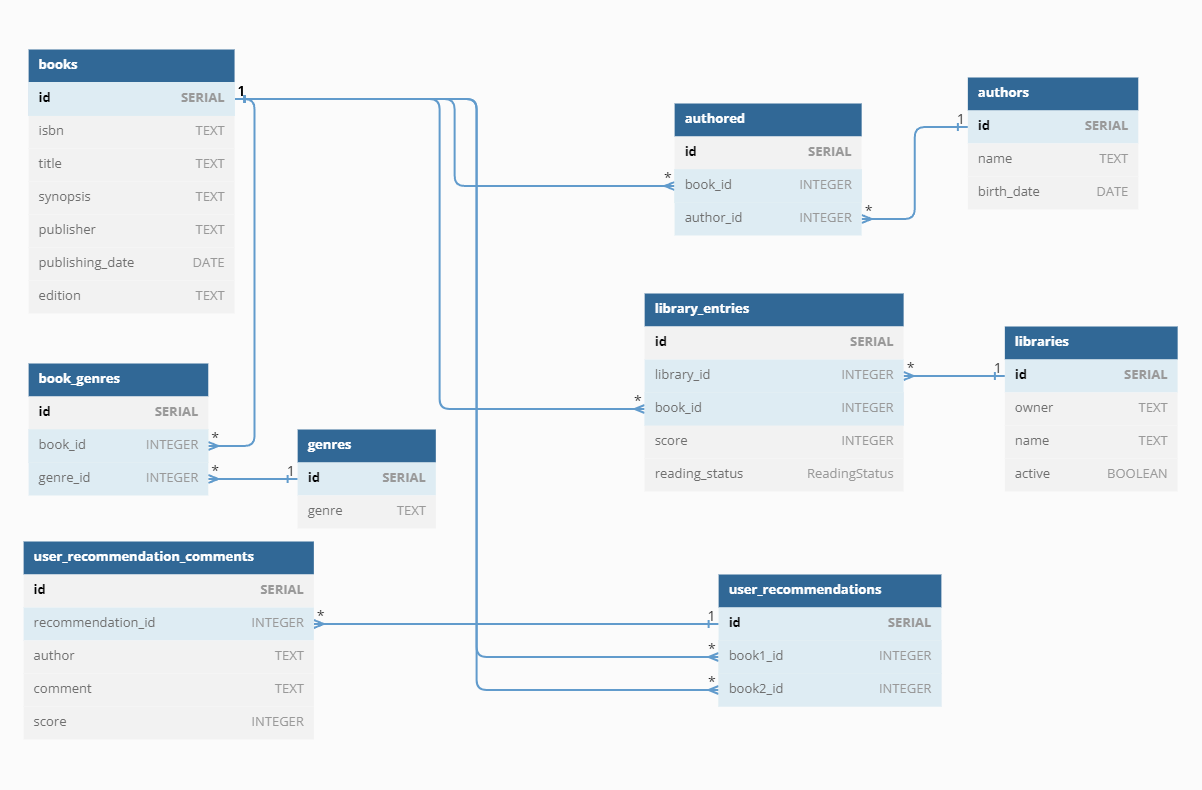
\includegraphics[width=0.9\textwidth]{img/diagrama_bd.png}\\[1.4cm]

El diagrama anterior se ha generado con \href{https://dbdiagram.io/}{dbdiagram.io}, web que permite importar scripts en diversos lenguajes de bases de datos y generar un diagrama automáticamente.

Nótese que el identificador del libro no es el ISBN, como uno podría esperar. Esto se debe a que aunque el ISBN debería ser único, a veces las editoriales cometen el error de asignar el mismo ISBN a dos o más títulos, o incluso se emplean intencionadamente para identificar colecciones de libros. Por otra parte, este identificador es de uso comercial, lo que quiere decir que no tiene por qué estar presente en libros que no hayan sido puestos a la venta. Estos motivos han llevado a la decisión de que el identificador de un libro debe ser otro, en este caso, un serial interno, y que la duplicidad o ausencia del ISBN debe ser soportada.

\subsubsection{Gestor de datos}

La primera implementación de la API se introdujo en el segundo PMV (ver \nameref{pmv2}). En este momento, al ser una fase temprana del proyecto, se carecía de una base de datos, por lo que para poner este código a prueba se introdujeron datos de prueba y lógica en la propia API, aunque esto incumpla el principio de responsabilidad única.

En esta primera versión de la API, cada \textit{endpoint} consultaba los datos almacenados en una variable global, realizaba las operaciones necesarias sobre estos y devolvía la respuesta con el mero objetivo de pasar los tests, pues en este momento no había base de datos como para ofrecer una funcionalidad real. Siguiendo el principio de responsabilidad única, el único trabajo del que debería encargarse la API es de recibir peticiones, delegar las acciones requeridas a otros módulos y devolver la respuesta correspondiente.

Fue a continuación, en el tercer PMV (ver \nameref{pmv3}) cuando se trabajó en solventar esta situación. Con un nuevo módulo llamado \textit{Data Manager} (Gestor de Datos) se movió todo el apartado de consulta de datos fuera de la API. Este gestor de datos se encarga de establecer una conexión con una base de datos, realizar una consulta determinada y devolver la información a la API, que ya se encargaría de delegar el procesamiento de está información a otros módulos según fuera necesario.

Dado que la implementación de la base de datos fue uno de los últimos pasos de este PMV, al principio se seguían usando datos de pruebas almacenados en esta clase gestora. Sin embargo su implementación sí que pretendía emular una conexión con una base de datos, realizando la conexión a esta al principio de cada consulta y cerrándola siempre al final.

En este punto se detectó un problema. Fue necesario refactorizar gran parte del código, pues hubo que llevar mucha funcionalidad de la API a esta nueva clase gestora. Esto planteó dudas sobre si la planificación del desarrollo de esta parte fue correcta.

Esto no habría ocurrido si se hubiese desarrollado la base de datos en primer lugar, seguida de la clase gestora de datos y finalmente por la API. Por un momento al pensar en este nuevo orden de desarrollo sentí que había cometido un error notable, pero dicha sensación se esfumó al pensar que, con la cantidad de trabajo que esas partes hubieron requerido, no habría conseguido realizar ninguna entrega funcional a un supuesto cliente en mucho tiempo ya que nada de esto aportaría utilidades nuevas hasta que la API no estuviera incluida, y esto no encaja con la mentalidad ágil propuesta para este desarrollo.

La versión final de este gestor de datos se conecta a la base de datos con información leída de las variables de entorno. En ficheros de tipo \textit{.env} se definen las diferentes variables necesarias para realizar la conexión a la base de datos: \textit{HOST, DATABASE, USER, PASSWORD, PORT}. Al momento de ejecutar la aplicación, dado que se está usando \textit{Poetry}, se puede indicar el \textit{path} del fichero \textit{.env} como valor de la variable \textit{POETRY_DOTENV_LOCATION}. 

En pocas palabras, indicamos el fichero con las variables de entorno que usará la aplicación. De esta forma es muy fácil tener varios de estos ficheros para diferentes bases de datos a las que conectar. Un ejemplo práctico que demuestra la utilidad de esta forma de hacerlo es tener dos de estos ficheros, uno orientado a una base de datos de producción, y otro a una base de datos de \textit{testing}. En el \href{https://github.com/Anglepi/My-Many-Reads/blob/main/Makefile}{\textit{Makefile}} del proyecto se puede ver como se hace uso de \textit{test.env} para la ejecución de \textit{tests} mientras que se usa \textit{prod.env} para la ejecución normal de la aplicación.

Dado que la información de conexión es sensible, no se encuentra en el repositorio ni es visible en el código. Esta es otra de las ventajas de usar ficheros de entorno para almacenar y ocultar esta información.

\subsection{Sistema de recomendaciones}

Este sistema es uno de los puntos más importantes del proyecto, pues es el que más atractivo aporta con respecto a los usuarios. Se compone, básicamente, de dos subsistemas: recomendaciones automáticas basadas en librerías y recomendaciones creadas por usuarios.

\subsubsection{Recomendaciones de los usuarios}

Para cada pareja de libros, los usuarios podrán escribir un comentario para justificar la recomendación entre ambos libros. Otros usuarios podrán votar dichos comentarios con el fin de apoyar esa recomendación.

El primer paso será determinar cual puede ser la mejor estructura de datos para esta situación. Por una parte, los libros ya se encuentran almacenados en el sistema, por lo que incluirlos de nuevo sería redundante, con su identificador será suficiente.

En este punto ya hay que tener en cuenta algunos aspectos importantes:

\begin{enumerate}
    \item No tiene sentido recomendar un libro consigo mismo.
    \item Recomendar el libro A con el libro B es igual que recomendar el libro B con el libro A
    \item Las recomendaciones son únicas, es decir, para una pareja de libros habrá uno o varios comentarios de usuarios, pero una única instancia de la pareja.
    \item Un usuario no puede escribir más de una recomendación por pareja de libros, pues no tendría sentido.
\end{enumerate}

El primer punto es sencillo de tratar, con comprobar que la pareja de libros introducida no está formada por un único identificador duplicado, el problema se soluciona.

Con respecto al segundo punto, lo ideal sería encontrar una estructura de datos predefinida que permitiera crear parejas de objetos las cuales no estuvieran ordenadas, pero no hubo mucha suerte al buscar esto para Python, por lo que simplemente se ordena la tupla al almacenarla para facilitar la comprobación.

Lidiar con el tercer punto es bastante sencillo una vez se ha definido la situación en lenguaje natural. Al crear una recomendación habrá que comprobar si la pareja indicada de libros ya tenía otras recomendaciones o no. En caso afirmativo bastará con añadir el comentario especificado a ésta, y en caso negativo se creará la pareja a la que se le añadirá dicho comentario.

Finalmente, el último punto está bastante relacionado con el anterior. De la naturaleza de estas recomendaciones se comienza a sobreentender que para cada pareja de libros existe una lista de comentarios escritos por usuarios, por lo que lo único necesario a realizar será, en el momento de añadir un nuevo comentario, comprobar que de los ya existentes la lista correspondiente ninguno pertenece al nuevo autor.

Con toda esta lógica ya controlada e incluida, el único aspecto a controlar es el de la votación, la cual tiene un proceso bastante sencillo, simplemente identificar el comentario objetivo e incrementar en uno su puntuación. Este proceso ganará en complejidad una vez se implementen las sesiones de usuarios, ya que habría que controlar que comentarios ha votado el usuario identificado con el fin de permitir que solo pueda votar una vez por comentario.

\subsubsection{Recomendaciones automáticas}

Para elaborar un algoritmo que pueda hacer sugerencias de manera automática para los usuarios, es necesario en primer lugar ser capaz de determinar los gustos de dicho usuario. Para ello, dado que un usuario puede organizar sus lecturas en varias bibliotecas, se van a generar las recomendaciones en base a los gustos definidos en una biblioteca específica, aportando mayor versatilidad a los usuarios de cara a la búsqueda de nuevas lecturas.

Este algoritmo de recomendaciones ofrece como resultado una lista de libros ordenados de mayor a menor relevancia con respecto a la biblioteca especificada. Para construir esta lista se sigue un proceso que puede dividirse en tres pasos principales:

\begin{enumerate}
    \item Se generan unas características generales de una biblioteca objetivo, agrupando todas las características relevantes de los libros que la componen con el fin de calcular la afinidad de un libro respecto a ésta. Dos de las características más evidentes de un libro que pueden usarse para esta tarea son los géneros y los autores, ya que a partir de éstas se puede definir muy bien la temática de un libro y su estilo de escritura. Para hacer esta recopilación de características, se puede realizar un conteo de todos los géneros y autores pertenecientes a cada libro, ponderando cada una de estas apariciones con un valor derivado de la puntuación que el usuario dueño de esa biblioteca ha asignado al libro en concreto, ayudando así a resaltar los géneros y autores favoritos.
    \item Mediante una función capaz de comparar un libro con estas características recopiladas, se otorga una puntuación de compatibilidad de un libro objetivo con respecto a una biblioteca, que hace las veces de correlación. Esta función comparará las propiedades del libro con las de las características recogidas, siempre teniendo en cuenta que no todas estas características son igual de valiosas para este proceso. Por ejemplo, los géneros de un libro son más representativos que, por ejemplo, la editorial.
    \item Finalmente, con las características de una biblioteca y la función para puntuar libros respecto a estas se puede generar la lista de recomendaciones. Para ello, se filtra la lista de libros candidatos, pues debemos eliminar los que ya se encuentren en la biblioteca, y se puntúa cada uno de los restantes. Para construir el resultado, estos libros se ordenan por puntuación, facilitando así devolver un subconjunto de los más relevantes.
\end{enumerate}

Para medir la compatibilidad se pueden tener en cuenta una gran cantidad de propiedades de los libros, no solo géneros y autores, sino también fecha de publicación, similitudes entre las sinopsis, apariciones en bibliotecas similares de otros usuarios e incluso según las recomendaciones manuales.

Conociendo ya todos estos aspectos, solo resta hacer algo de experimentación jugando con la inclusión de algunos o todos éstos parámetros y ajustando sus pesos hasta dar con un modelo satisfactorio.